\subsection{Fyzicka implementace}
Fyzická implementace definuje \textbf{datové struktury} pro základní logické objekty:

\begin{itemize}
\item \textbf{tabulky},
\item \textbf{indexy},
\item \textbf{materializované pohledy} (materialized views),
\item \textbf{rozdělení dat} (data partitioning) --  data s dlouhou historií. Fyzické rozdělení datových struktur a souboru na více částí.
\end{itemize}

Fyzická implementace tedy \textbf{řeší uložení dat na nejnižší úrovni databáze}.
 Na úrovni databáze můžeme ovlivnit výběr efektivnějšího plánu vykonávání dotazu případně \textbf{dobu vykonávání operací}.

\begin{itemize}
\item \textbf{ROWID} -- jedinečné číslo \textbf{označující záznam tabulky}.
\item Větší část teorie fyzického návrhu DB je platná pro libovolné SŘBD, dále se musíme řídit \textbf{doporučením výrobce}.
\item Každé SŘBD obsahuje specifickou reprezentaci tabulek a indexů:
\begin{itemize}
\item \textbf{CREATE TABLE} - vytvoření tabulky typu \textbf{halda} (Oracle), \textbf{shlukování záznamů} (SQL Server 2012).
\item \textbf{CREATE INDEX} - vytvoření\textbf{ B+-stromu}, kde každá položka odkazuje na ROWID záznamu v tabulce.
\end{itemize}
\end{itemize}

\subsection{Datové struktury}
Datové struktury \textbf{se skládají} buďto ze \textbf{stránek}, nebo z \textbf{uzlů} v případě stromové struktury. Jejich realizace přímo ovlivňuje efektivitu \textbf{operací} vyhledávání, vkládání, editace a mazání. Konkrétní realizace je závislá na použitém typu tabulky (halda, halda+index, shlukování záznamů).

Základní datové struktury:
\begin{itemize}
\item \textbf{Blok} (alokační jednotka) -- je nejmenší jednotka, se kterou SŘBD manipuluje při zápisu a čtení dat z disku (obvykle 4KB nebo 8KB).
\item \textbf{Stránka} -- nejmenší jednotka s kterou pracuje správce paměti. \texttt{Stranka.velikost = X * Blok.velikost} (je-li velikost bloku = 4KB je odpovídá velikost stránky násobkům 4KB).
\item \textbf{Datový soubor} -- fyzický prostor na disku s daty.
\end{itemize}


\subsection{Typy tabulek}
\subsubsection{Heap Table}
\begin{itemize}
\item Implicitní pro \texttt{CREATE TABLE} téměř všude, pokud tabulka nemá žádné indexy (ani PK). Záznamy nejsou nijak uspořádány.
\item \textbf{Stránkové perzistentní pole} s velikostí \textbf{bloku} nejčastěji \textbf{8kB}.
\item Záznamy pouze \textbf{označovány jako smazané}, pro fyzické smazání slouží speciální operace \textbf{shrinking}.
\item Obsahuje všechny záznamy a jejich atributy pokupě.
\item Při vkládání záznam uložen na \textbf{první volnou pozici v tabulce} nebo na \textbf{konec pole}.
\item Složitost operací: neefektivní vyhledávání $O(n)$, velmi \textbf{efektivní vkládání} $O(1)$ i \textbf{využití místa}.
\end{itemize}
\subsubsection{Shlukování záznamů (Data Clustering)}
\begin{itemize}
\item Implicitní pro MS-SQL při \texttt{CREATE TABLE}
\item Záznamy v \textbf{datovém souboru jsou seřazeny podle zvoleného klíče}, pro implementaci nejčastěji využita nějaká \textbf{varianta B-stromu}.
\item Listové uzly stromu (bloky) obsahují \textbf{kromě klíče i další atributy} tabulky.
\item V pokročilejších DBMS lze zvolit, které atributy leží přímo v B+ stromu a které leží na haldě. Lze tak kombinovat shlukování s heap table. Pro získání dat uložených přímo v listu není přístup na haldu poté nutný
\item Používá se všude, kde potřebujeme \textbf{získat i hodnoty ostatních atributů} (kromě klíče - např. \texttt{SELECT} neklíčových atributů) - vyšší výkon
\item \textbf{Zhoršený výkon} \texttt{INSERT} (data se musí zatřizovat).
\item \textbf{Oracle:} Index Organized Table (IOT), \textbf{SQL Server:} Clustered Index.
\end{itemize}

\paragraph{Eliminace náhodných přístupů přes ROWID} Tabulka se shlukováním záznamů může ušetřit náhodný přístup oproti heap table a indexu. Po vyhledání ve stromě není nutné další náhodný přístup na haldu, protože vše potřebné je v listu. Kvůli více datům v listech může ale být celková výška stromu ve shlukované tabulce mnohem větší. To způsobí více náhodných přístupů při průchodu stromem než  v případě heap table a indexu. Co je lepší nelze určit předem ale pouze testem na reálných nebo pseudoreálných datech.

\subsubsection{Hašovaná tabulka (Hash Table)}
\begin{itemize}
\item Záznamy se stejnou hashovanou hodnou jsou uloženy ve stejném nebo velmi blízkém bloku.
\item Trochu \textbf{plýtvá místem}.
\item Musíme znát předem velikost záznamů (alespoň přibližně).
\end{itemize}

\subsubsection{Materializované pohled (Materialized views)}
\begin{itemize}
\item Uložené \textbf{výsledky dotazů}, které bývají často v DB vyhodnocovány.
\item Jde spíše o \textbf{fragment} z \textbf{tabulky} či několika tabulek.
\end{itemize}

\subsection{Indexy}
Indexové soubory slouží k možnosti \textbf{rychlého vyhledávání a seřazení tabulky} podle různých atributů. Tabulka je jinak seřazena úplně náhodně (heap table), nebo podle primárního klíče (data-clustering). Index je tedy vázaný ke konkrétní tabulce a konkrétnímu atributu. Index umožňuje \textbf{rychlé vyhledávání} dle klíče, \textbf{ROWID pak odkazuje na kompletní záznam v heap tabulce}. \texttt{CREATE [BITMAP] INDEX login ON Student;}. Protože ale následný počet náhodných přístupů pomocí ROWID může být mnoho, někdy DB raději provede sekvenční prohledání celé tabulky. Rozhoduje se individuálně na základě statistik o atributech a jejich velikostech.
\begin{itemize}
\item \textbf{Primární index (PRIMARY)} -- automatický index, který se váže k primárnímu klíči, zajišťuje jedinečnost údajů.
\item \textbf{Unikátní index (UNIQUE)} -- stejně jako primární index zajišťuje jedinečnost údajů v atributu, ale neváže se k primárnímu klíči.
\item \textbf{Vedlejší index (INDEX)} -- klasické index popsány níže.
\item \textbf{Fulltextový index} -- používá se pro optimalizaci fulltextového vyhledávání v daném sloupci.
\item \textbf{Složený index} -- Může být kterýkoli výše. Obsahuje více atributů v jednom klíči. Pokud je dotaz jen na druhý či další atribut v indexu, nelze index použít.
\end{itemize}

\subsubsection{Nevýhody indexů}
\begin{itemize}
	\item Při velkém množství různých indexů mohou soubory s index zabírat mnohem více než samotná tabulka
	\item Pro získání dalších dat je nutné hodně náhodných přístupů přes ROWID
	\item Každý záznam v indexu musí být shodné délku. Tj například stringy nejsou vhodné pro index, protože každý záznam v indexu bude tak dlouhý, jaký je nejdelší možný string daného atributu. Pokud je string kratší, je záznam v indexu vyplněn \texttt{\\0}.
\end{itemize}

\subsubsection{Bitmapový index}
\textbf{Odpovídá na všechny možné hodnoty daného atributu}. Jde o tabulku jedniček a nul, kde řádky reprezentují záznamy v indexované tabulce a sloupce hodnoty indexovaného atributu. Jednička pak znamená true, že záznam má hodnotu danou sloupcem. \textbf{Vyplatí se}, pokud se používají logické operátory (\texttt{AND}, \texttt{OR}, \texttt{XOR}) \textbf{nad několika bitmapovými indexy atributů}.

\begin{figure}[H]
	\centering
	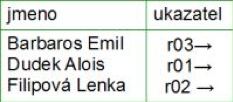
\includegraphics[width=0.3\textwidth]{assets/index_classic.png}
	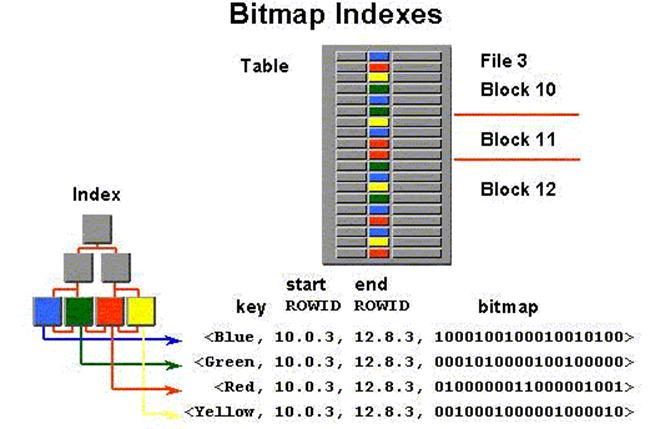
\includegraphics[width=0.65\textwidth]{assets/index_bitmap.jpg}
\end{figure}

\subsubsection{Shlukovaný index (Cluster Index)}
Pokud se pro dvě tabulky často používá operace spojeni (JOIN) pro jeden atribut. V tomto případě diskový blok obsahuje záznam z řídicí tabulky a zároveň i závislé záznamy. (v normalnim připadě obsahuje diskovy blok pouze zaznamy jedne tabulky).

\subsubsection{Kandidáti na index}
\begin{itemize}
\item \textbf{Primární} klíče a \textbf{cizí} klíče.
\item Pokud je index používán pro nalezení malého počtu záznamů.
\item Pokud index pokryje jeden nebo více častých dotazů.
\item Atributy často se vyskytující v konstrukci \texttt{WHERE}.
\end{itemize}

\subsection{Vykonávání dotazu}
\textbf{Ovlivnění času vykonávání dotazu} - parametrizované dotazy, hromadné operace, nastavení transakcí. Na úrovni DB můžeme ovlivnit výběr efektivnějšího plánu vykonávání dotazu, případně dobu vykonávání operací -> \textbf{fyzický návrh DB}. Identifikujeme \textbf{4 fáze vykonávání dotazu}:

\begin{enumerate}
	\item \textbf{Parsování dorazu}
	\begin{itemize}
		\item Převod původního dotazu do zvolené \textbf{interní formy}.
		\item \textbf{Eliminujeme syntaxi jazyka dotazu} (např. SQL).
		\item Zpracování pohledů, které probíhá v této fázi, znamená, že \textbf{nahradíme pohled jeho definicí} (materializované pohledy -- fragmenty/výsledky dotazů).
		\item Interní forma je nejčastěji \textbf{nějaký druh dotazovacího stromu} (angl. query tree).
	\end{itemize}
	\item \textbf{Výběr logického plánu}
	\begin{itemize}
		\item při převodu do formy relační algebry dochází také k \textbf{odstranění} různých povrchních \textbf{rozdílů} a především nalezení \textbf{efektivnějšího} \textbf{tvaru} než nabízel původní dotaz.
		\item \textbf{Optimalizátor} – transformační pravidla (převádí výraz na ekvivalentní). Fáze transformace/přepsání dotazu (query rewite). Dotaz tedy není ve skutečnosti vykonán přesně tak, jak byl zadán! 
	\end{itemize}
	\item \textbf{Výběr fyzického plánu}
	\begin{itemize}
		\item V této fázi se optimalizátor rozhoduje jak bude transformovaný dotaz vykonán.
		\item Jsou vybírány konkrétní algoritmy a pořadí jejich vykonávání.
		\item Při výběru se již uvažuje: \textbf{existenci indexů}, \textbf{distribuci hodnot}, \textbf{shlukování uložených dat}.
		\item Každé operaci je přiřazena výsledná \textbf{cena = IO cost + CPU cost}, která bude potřebná k celkovému vykonání.
	\end{itemize}
	\item \textbf{Výběr nejlevnějšího plánu a jeho vykonání}
	\begin{itemize}		
		\item Z množiny dotazovacích plánů pak \textbf{optimalizátor} vybírá ten \textbf{nejlepší}, tedy \textbf{nejlevnější} plán.
		\item Následně je vykonán a hodnoty vráceny.
	\end{itemize}
\end{enumerate}

\begin{figure}[H]
	\centering
	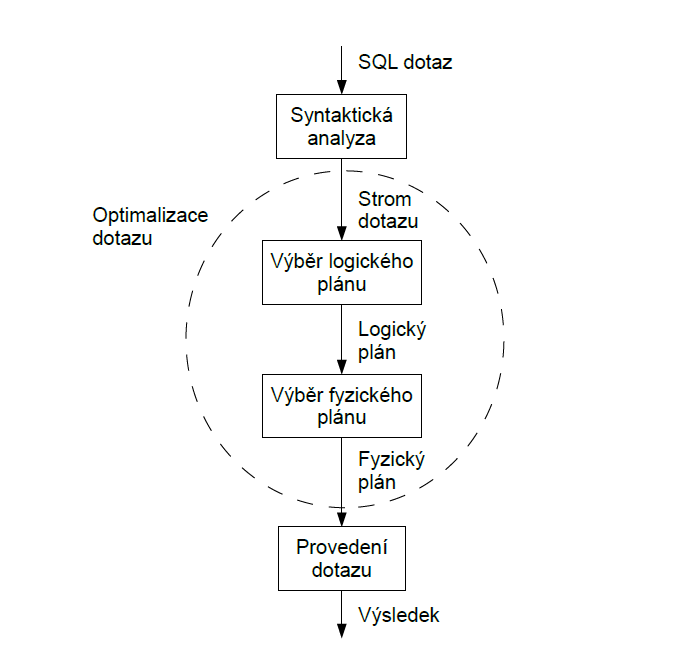
\includegraphics[width=0.6\textwidth]{assets/zpracovani_dotazu.png}
\end{figure}

\subsection{Optimalizátor a ladění dotazů}
\begin{itemize}
	\item \textbf{Optimalizátor} pro nalezení nejlepšího plánu využívá systémový katalog, který obsahuje statistiky o uložených datech. Systémový katalog je aktualizován v době nejnižší zátěže serveru, nikoli po každé CRUD operaci. Orientační obsah katalogu:
	\begin{itemize}
		\item \textbf{Tabulka} - kardinalita (mohutnost, počet záznamů), počet diskových stránek
		\item \textbf{Sloupec} - počet stejných hodnot ve sloupci, minimální a maximální hodnoty, null hodnoty, $X$ nejfrekventovanějších hodnot
		\item \textbf{Index} - Počet listových stránek, výška stromu
	\end{itemize}
	\item \textbf{Plán} lze v SŘBD většinou \textbf{zobrazit} - operace jako průchod tabulkou, přístup k indexu, třídění spojení atd. To lze využít pro \textbf{odladění dotazu} - např. uvidíme, že musíme použít index na neindexovaný atribut.
	\item Dvěma či více \textbf{různými dotazy} je možno obdržet \textbf{stejná data}. 
	\item \textbf{Rychlost} různých dotazů ovšem\textbf{ nemusí být stejná }i přesto, že vracejí stejná data.
	\item Snažíme dosáhnout \textbf{maximálního} \textbf{výkonu} se \textbf{stávajícími prostředky}.
	\item Snažíme se vytvořit dotaz, který\textbf{ bude načítat z úložiště pouze to, co potřebuje}.
\end{itemize}

\subsubsection{Přístupy k ladění}
\begin{itemize}
\item \textbf{Proaktivní} -- Analyzujeme fyzický návrh a provádíme změny k lepšímu fungování.
\item \textbf{Reaktivní} -- Reagujeme na problém.
\end{itemize}

\subsubsection{Ladění výkonu SŘBD}
\begin{itemize}
	\item \textbf{HW} -- RAID, RAM, CPU (Poslení možnost, je to drahé, efektivnější je \textbf{vyladit fyzický návrh}).
	\item \textbf{Parametry SŘBD} -- Velikosti \textbf{cache}, maximum zámků, atd. Nutné optimalizovat na určité použití.
	\item \textbf{ORM} -- Minimum SQL příkazů a objemu přenášených dat. Úroveň izolace transakce.
\end{itemize}

\subsubsection{Obsah plánu vykonání dotazu}
V plánu lze získat informace:
\begin{itemize}
	\item \textbf{consisteng gets}  - logické přístupy + počet záznamů výsledků/velikost pole záznamů,
	\item \textbf{physical reads} - fyzické čtení,
	\item \textbf{sorts(memory)} - počet operací třízení, bez přístupu na disk,
	\item \textbf{sorts(disk)} - počet operací s nejměně jedním přístupem na disk,
	\item pokud pro logický přístup neexistuje fyzický => \textbf{cache hit} (cache hit rate = (cache hit / počet logických čtení) * 100 [\%]
	\item opačný případ \textbf{cache miss},
	\item vhodné sledovat i další parametry \textbf{Bytes received from server}, \textbf{Total execution time}.
\end{itemize}

\begin{figure}[H]
	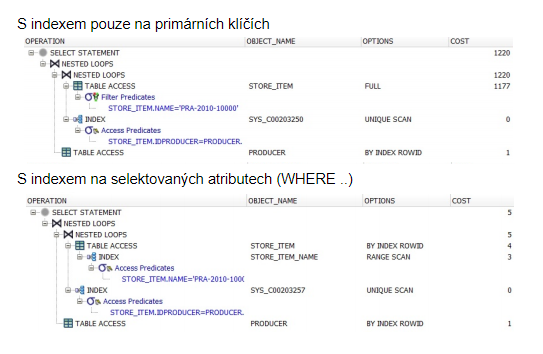
\includegraphics{assets/plan_vykonani_dotazu_oracle.png}
\end{figure}